\documentclass[10pt,a4paper,oneside]{article}
\usepackage{cmap}
\usepackage[T2A]{fontenc}
\usepackage{float}
\usepackage{listings}
\usepackage{csquotes}
\usepackage[utf8]{inputenc}
\usepackage{amsmath}
\usepackage{amsfonts}
\usepackage{amssymb}
\usepackage[english, russian]{babel}%Подключаем русский язык.
\usepackage{graphicx}
\usepackage{geometry} % Меняем поля страницы.
\geometry{left=3cm} %Левое поле.
\geometry{right=2cm} %Правое поле.
\geometry{top=3cm} %Верхнее поле.
\geometry{bottom=2cm} %Нижнее поле.


%Начало документа
\begin{document}

%Создаём титульник.
\begin{titlepage}
\newpage
	%Название ВУЗа и институт.
	\begin{center}
		\Large Санкт-Петербургский Государственный Политехнический Университет\\
		Институт Компьютерных Наук и Технологий\\
	\end{center}
	%Кафедра.
	\begin{center}
		\large\textbf {Высшая школа интеллектуальных систем и суперкомпьютерных технологий}
	\end{center}
	
	%Пропуск места. 
	\vspace{5em}
	%!!!!!!!!!!!!!!!!!!!!!!!!!!!!!!!!!Название работы.
	\begin{center}
		\large{Отчёт по лабораторной работе №11 \\ на тему \\
		\textbf{Модуляция и выборка} }
	\end{center}
	
	%Делаем пропуск и пишем студента и преподавателя.
	\vspace{25em}
	\begin{flushright}
		\textbf{Работу выполнил\\}Студент группы 3530901/80203 \\ Тарасенко Н.С.\\
		\textbf{Преподаватель\\}Богач Н.В. 
	\end{flushright}
	
	\vspace{\fill}%В самом низу
	\begin{center}
	Санкт-Петербург, 2021 год	
	\end{center}
\end{titlepage} %Закончили титульный лист.

\section{Цели:}
    -Поймите проблемы искажения сигнала и эффектов канала.

-Определите этапы, необходимые для восстановления сигналов.

    -Сроки восстановления
    
    -Многолучевые каналы
    
    -Фазовая и частотная коррекция
    
    -Декодирование символов и порядок битов
    

\section{Передача сигнала:}
Первый этап - передача сигнала QPSK. Мы генерируем поток битов и модулируем его на сложное созвездие. Для этого мы используем блок Constellation Modulator , который использует Constellation Rect. Объект и другие настройки для управления передаваемым сигналом. Параметр Constellation Modulator - это идентификатор Constellation Rect. Object (qpsk_const), даже если он отображается на потоковом графике как что-то еще.

Объект созвездия позволяет нам определить, как кодируются символы. Затем блок модулятора может использовать эту схему модуляции с дифференциальным кодированием или без него. Модулятор созвездия ожидает упакованные байты, поэтому у нас есть генератор случайного источника, предоставляющий байты со значениями 0-255.

Имея дело с количеством выборок на символ, мы хотим, чтобы это значение было как можно меньшим (минимальное значение 2). Как правило, мы можем использовать это значение, чтобы помочь нам сопоставить желаемую скорость передачи данных с частотой дискретизации оборудования, которое мы будем использовать. Поскольку мы используем моделирование, количество отсчетов на символ важно только для того, чтобы обеспечить соответствие этой скорости по всей потоковой диаграмме. Мы будем использовать здесь 4, что больше, чем нам нужно, но полезно для визуализации сигнала в различных областях.

Наконец, мы устанавливаем значение избыточной пропускной способности. Модулятор созвездия использует фильтр формирования импульса с приподнятым косинусом (RRC), который дает нам единственный параметр для регулировки коэффициента спада фильтра, часто называемого математически «альфа». Поточный график mpsk_rrc_rolloff.grc ниже генерирует следующий рисунок, показывающий различные значения избыточной пропускной способности. Типичные значения находятся в диапазоне от 0,2 (красная кривая) до 0,35 (зеленая кривая).

\begin{figure}[H]
        \centering
        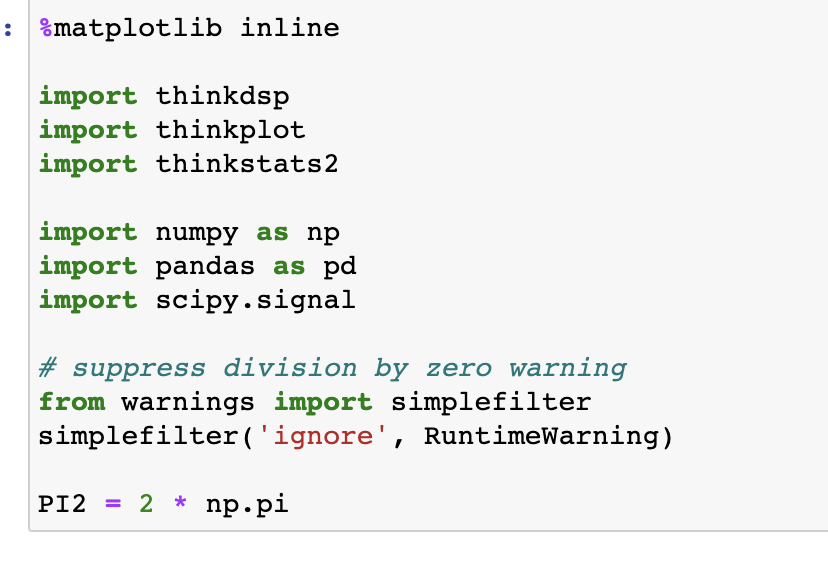
\includegraphics[width=0.75\textwidth]{0.png}
        \caption{2}
        \label{fig:first}
\end{figure}

\begin{figure}[H]
        \centering
        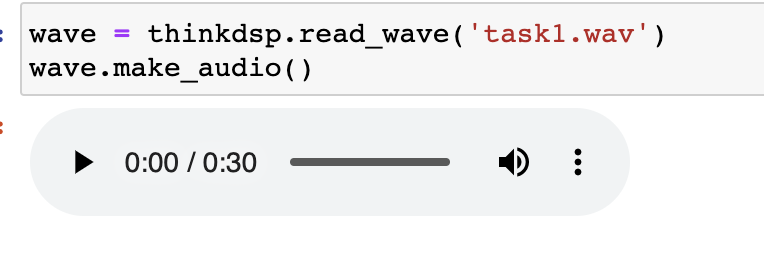
\includegraphics[width=0.75\textwidth]{1.png}
        \caption{2}
        \label{fig:first}
\end{figure}

Пример потокового графа mpsk_stage1.grc передает созвездие QPSK. Он отображает как передаваемый сигнал, так и часть цепи приемника во времени, частоте и диаграмме созвездия.

\begin{figure}[H]
        \centering
        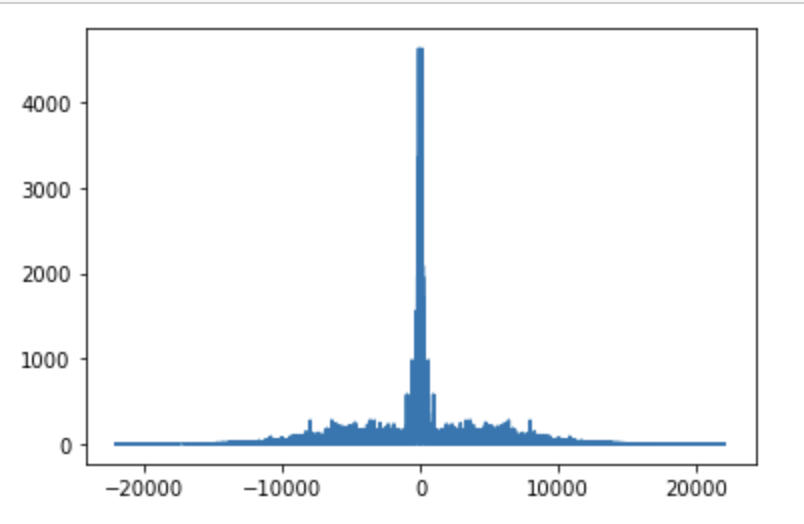
\includegraphics[width=0.75\textwidth]{2.png}
        \caption{2}
        \label{fig:first}
\end{figure}

На графике созвездия мы видим эффекты повышающей дискретизации(генерируя 4 отсчета на символ) и процесс фильтрации. В этом случае фильтр RRC добавляет преднамеренные самоинтерференции, известные как межсимвольные помехи (ISI). ISI плохо влияет на принимаемый сигнал, потому что смешивает символы. Мы рассмотрим это подробно во время раздела восстановления по времени. А сейчас давайте посмотрим, что мы делаем с сигналом. Если вы просто смотрите на передаваемые сигналы на этом графике, вы должны увидеть, что частотный график показывает сигнал красивой формы, переходящий в шум. Если бы мы не применили формирующий фильтр к сигналу, мы бы передавали прямоугольные волны, которые производили бы много энергии в соседних каналах. Благодаря уменьшению внеполосных излучений наш сигнал теперь остается в пределах полосы пропускания нашего канала.

\begin{figure}[H]
        \centering
        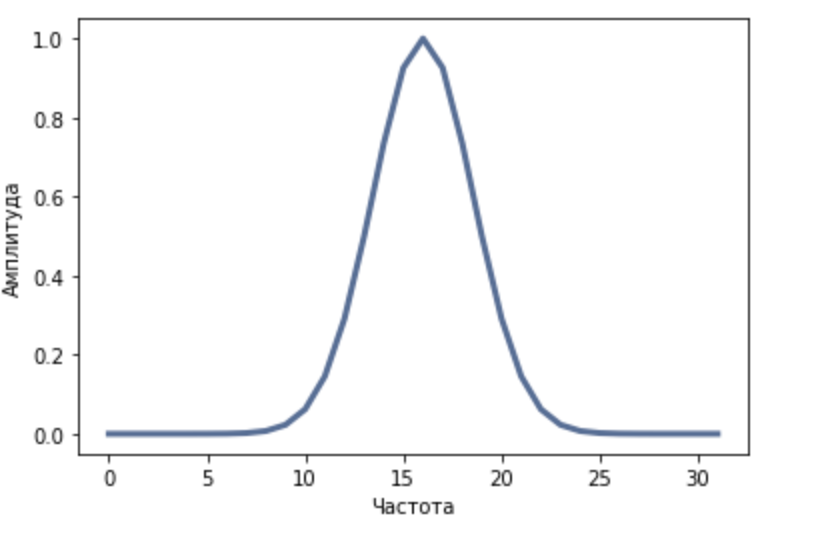
\includegraphics[width=0.75\textwidth]{3.png}
        \caption{2}
        \label{fig:first}
\end{figure}

На стороне приема мы избавляемся от ISI с помощью другого фильтра. По сути, то, что мы сделали, это целенаправленно использовали фильтр на передатчике, фильтр RRC, который создает ISI. Но когда мы сворачиваем два фильтра RRC вместе, мы получаем фильтр с приподнятым косинусом , который является формой фильтра Найквиста . Итак, зная это свойство фильтра RRC передачи, мы можем использовать другой фильтр RRC на приемнике. Фильтрация здесь просто свертка, поэтому выходной сигнал RRC-фильтра на приемной стороне представляет собой сигнал в форме приподнятого косинусоидального импульса с минимизированным ISI. Другое преимущество состоит в том, что при отсутствии эффектов канала мы используем согласованный фильтр на приемнике.

\section{Добавление нарушений канала:}

Этот пример первого этапа имел дело только с механикой передачи сигнала QPSK. Теперь мы рассмотрим влияние канала и то, как сигнал искажается между тем, когда он был передан, и тем, когда мы видим сигнал в приемнике. Первым шагом является добавление модели канала, что делается на примере mpsk_stage2.grc ниже. Для начала мы будем использовать самый простой блок модели канала GNU Radio.

Этот блок позволяет нам смоделировать несколько основных проблем, с которыми нам приходится иметь дело. Первая проблема с приемниками - это шум. Тепловой шум в нашем приемнике вызывает шум, который мы знаем как аддитивный белый гауссовский шум (AWGN) . Мы устанавливаем мощность шума, регулируя значение напряжения шума модели канала. Мы указываем здесь напряжение вместо мощности, потому что нам нужно знать полосу пропускания сигнала, чтобы правильно рассчитать мощность. Одним из определяющих аспектов GNU Radio является независимость блоков, поэтому модель канала ничего не знает о входящем сигнале. Мы можем рассчитать напряжение шума исходя из желаемого уровня мощности, зная другие параметры моделирования.

Второй этап нашего моделирования позволяет нам поиграть с этими эффектами аддитивного шума, сдвига частоты и временного сдвига. Когда мы запускаем этот график, мы добавили немного шума (0,2), некоторое смещение частоты 0,025) и некоторое смещение времени (1,0005), чтобы увидеть результирующий сигнал.

\begin{figure}[H]
        \centering
        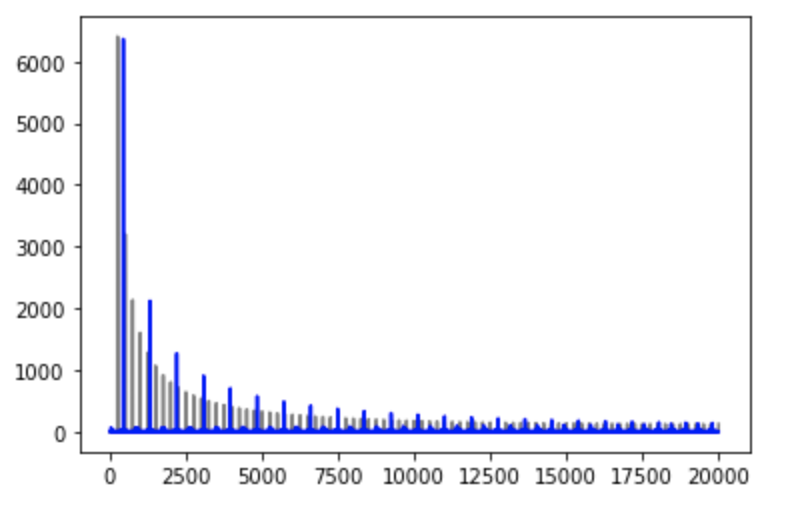
\includegraphics[width=0.75\textwidth]{4.png}
        \caption{2}
        \label{fig:first}
\end{figure}

\begin{figure}[H]
        \centering
        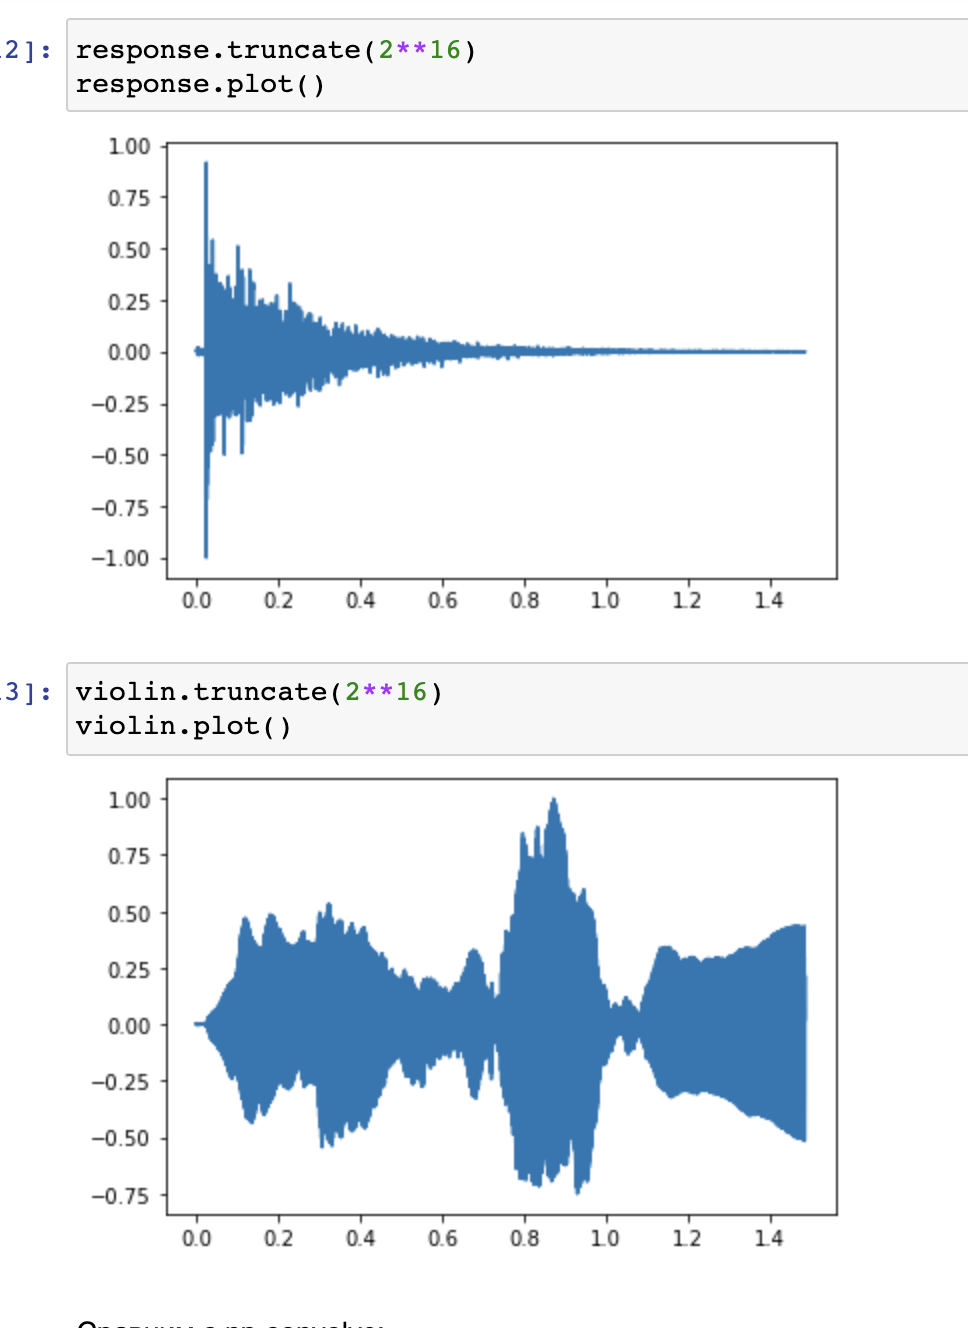
\includegraphics[width=0.75\textwidth]{5.png}
        \caption{2}
        \label{fig:first}
\end{figure}

График созвездия показывает нам облако образцов, намного худших, чем то, с чего мы начали на последнем этапе. Теперь, исходя из полученного сигнала, мы должны отменить все эти эффекты.

\section{Восстановление времени:}

Мы начнем с восстановления времени. Мы пытаемся найти наилучшее время для дискретизации входящих сигналов, что позволит максимизировать отношение сигнал / шум (SNR) каждой выборки, а также уменьшить влияние межсимвольной интерференции (ISI).

\begin{figure}[H]
        \centering
        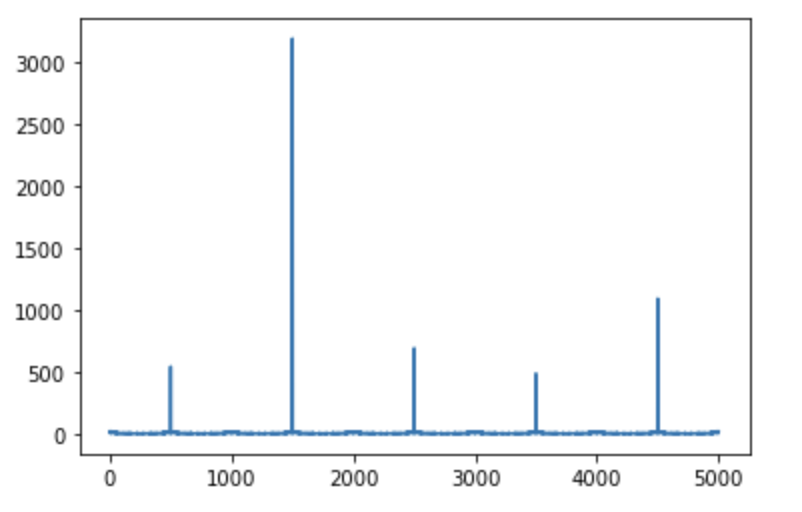
\includegraphics[width=0.75\textwidth]{6.png}
        \caption{2}
        \label{fig:first}
\end{figure}

\begin{figure}[H]
        \centering
        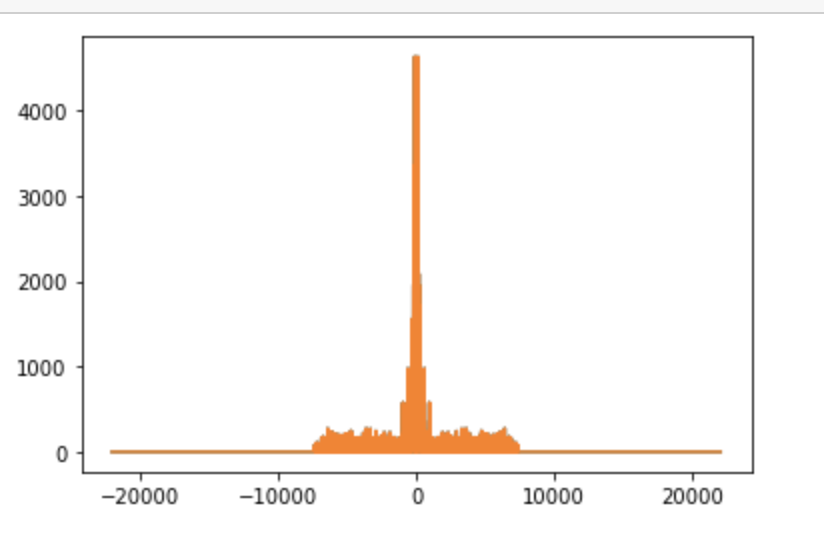
\includegraphics[width=0.75\textwidth]{7.png}
        \caption{2}
        \label{fig:first}
\end{figure}

Это моделирование позволяет нам легко настраивать такие вещи, как количество выборок на символ, избыточную полосу пропускания фильтров RRC и количество ответвлений. Затем мы можем поиграть с этими различными значениями, чтобы увидеть, как они влияют на поведение точки выборки.

Затем давайте посмотрим, что происходит из-за того, что разные часы влияют на точки выборки между передатчиком и приемником. Используя пример потокового графа в symbol_sampling_diff.grc, мы моделируем влияние разных часов в передатчике и приемнике. Все часы несовершенные, поэтому а) начнутся в другой момент времени и б) дрейфуют относительно других часов. Мы моделируем это, добавляя ресамплер, который немного регулирует время выборки символа между переданным сигналом (на переданном изображении выше) и приемником, показанным ниже. Показанная здесь разница часов в 1,125 является экстремальной как способ показать ее в этой настройке как метод визуализации. На самом деле разница во времени составляет порядка частей на миллион. Но здесь обратите внимание на то, что образцы, собираемые в разные моменты времени,

\begin{figure}[H]
        \centering
        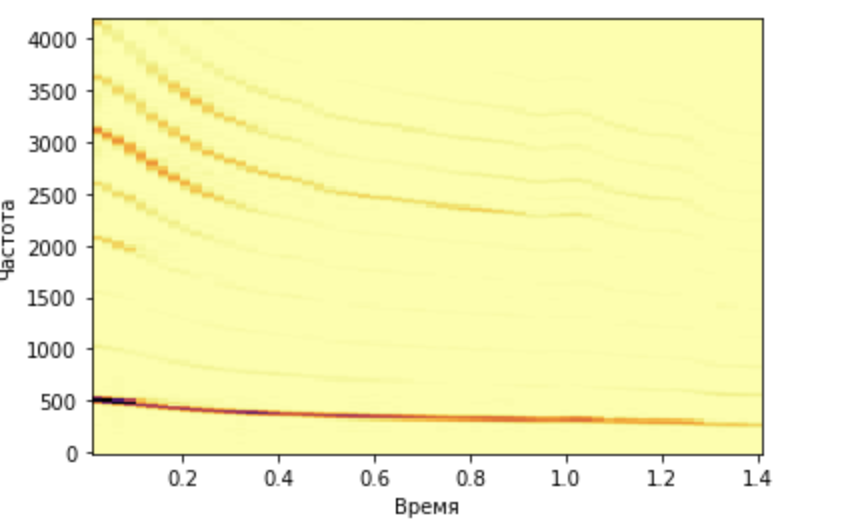
\includegraphics[width=0.75\textwidth]{8.png}
        \caption{2}
        \label{fig:first}
\end{figure}

\begin{figure}[H]
        \centering
        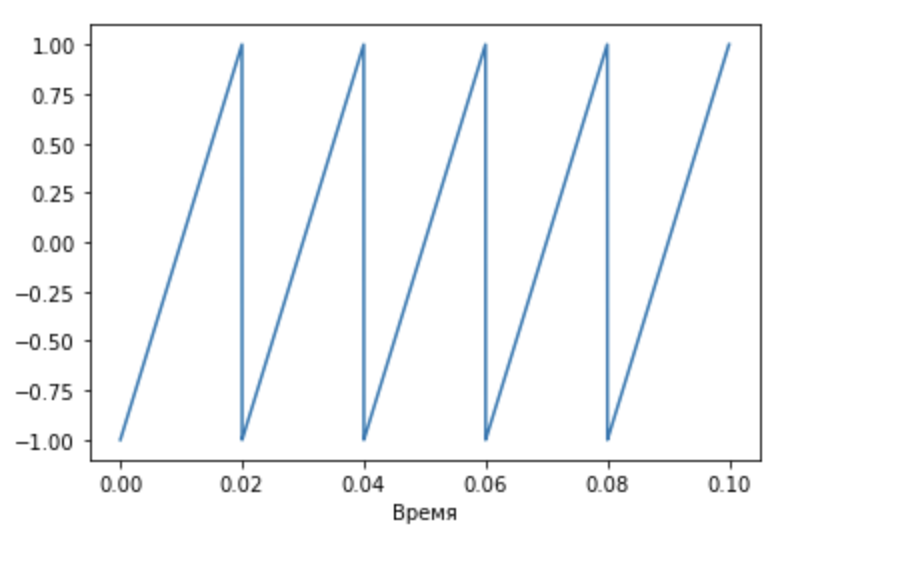
\includegraphics[width=0.75\textwidth]{9.png}
        \caption{2}
        \label{fig:first}
\end{figure}

Наша задача здесь - синхронизировать часы передачи и приемника, используя только информацию в приемнике из входящих выборок. Это задание известно как восстановление часов или времени.

\section{Блок многофазной тактовой синхронизации:}

Блок работает, вычисляя первый дифференциал входящего сигнала, который будет связан с его смещением тактовой частоты. Если сначала смоделировать это очень просто, мы увидим, как дифференциальный фильтр будет работать на нас. Во-первых, используя пример потокового графа symbol_differential_filter.grc, мы можем увидеть, как все выглядит идеально, когда наш параметр скорости равен 1 (т.е. нет смещения часов). Очевидно, что нам нужен образец 0,22 мс. Фильтр разности ([-1, 0, 1]) генерирует дифференциал символа, и, как показано на следующем рисунке, выходной сигнал этого фильтра в правильной точке выборки равен 0. Затем мы можем инвертировать этот оператор и вместо этого сказать, когда выход дифференциального фильтра равен 0, мы нашли оптимальную точку выборки.

\begin{figure}[H]
        \centering
        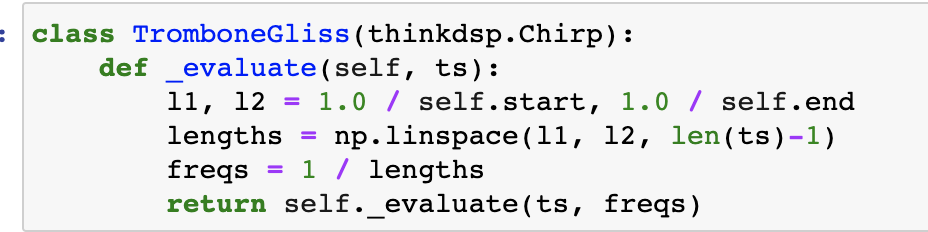
\includegraphics[width=0.75\textwidth]{10.png}
        \caption{2}
        \label{fig:first}
\end{figure}

\begin{figure}[H]
        \centering
        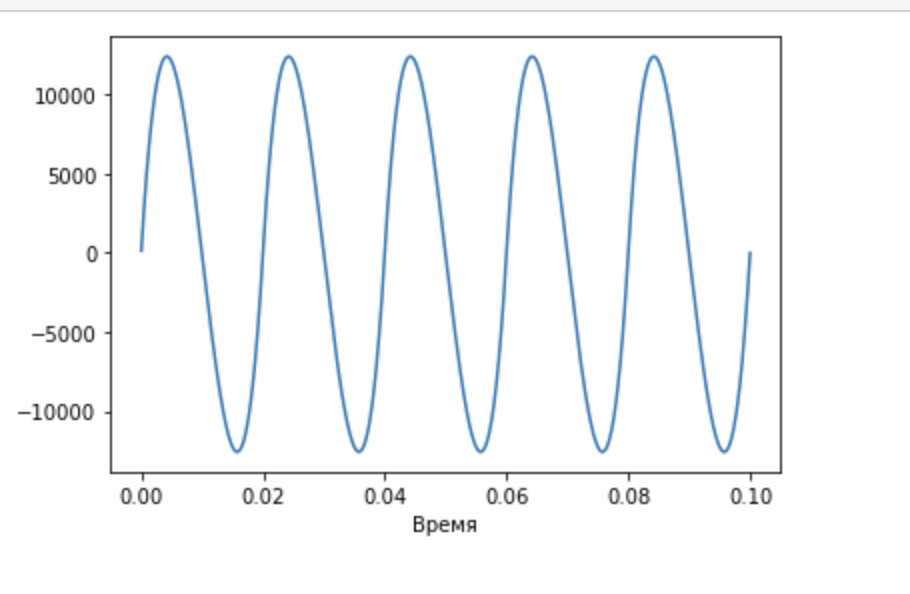
\includegraphics[width=0.75\textwidth]{11.png}
        \caption{2}
        \label{fig:first}
\end{figure}

Что происходит, когда у нас есть временное смещение? Этот результат, показанный ниже, показывает, что временное смещение, когда пик символа выключен, а производный фильтр не показывает нам нулевую точку.

\begin{figure}[H]
        \centering
        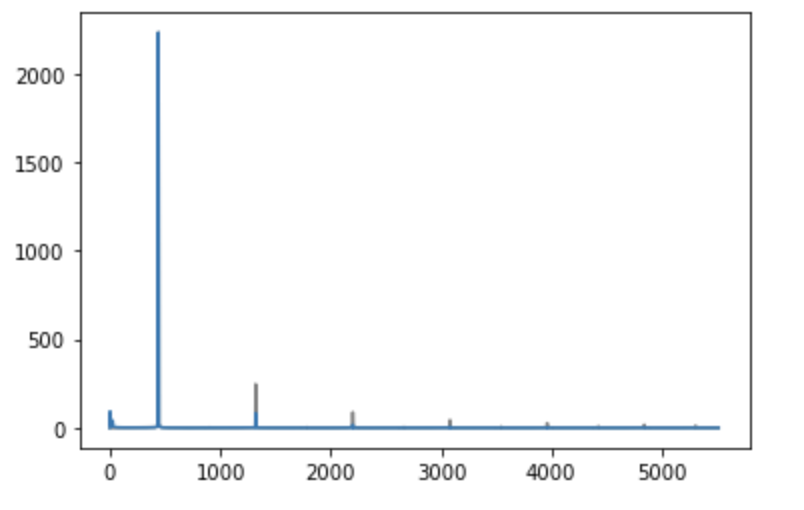
\includegraphics[width=0.75\textwidth]{12.png}
        \caption{2}
        \label{fig:first}
\end{figure}

Вместо использования одного фильтра мы можем создать серию фильтров, каждый с разной фазой. Если у нас достаточно фильтров на разных фазах, один из них - правильная фаза фильтра, которая даст нам желаемое значение синхронизации. Давайте посмотрим на симуляцию, которая строит 5 фильтров, что означает 5 различных фаз.

\begin{figure}[H]
        \centering
        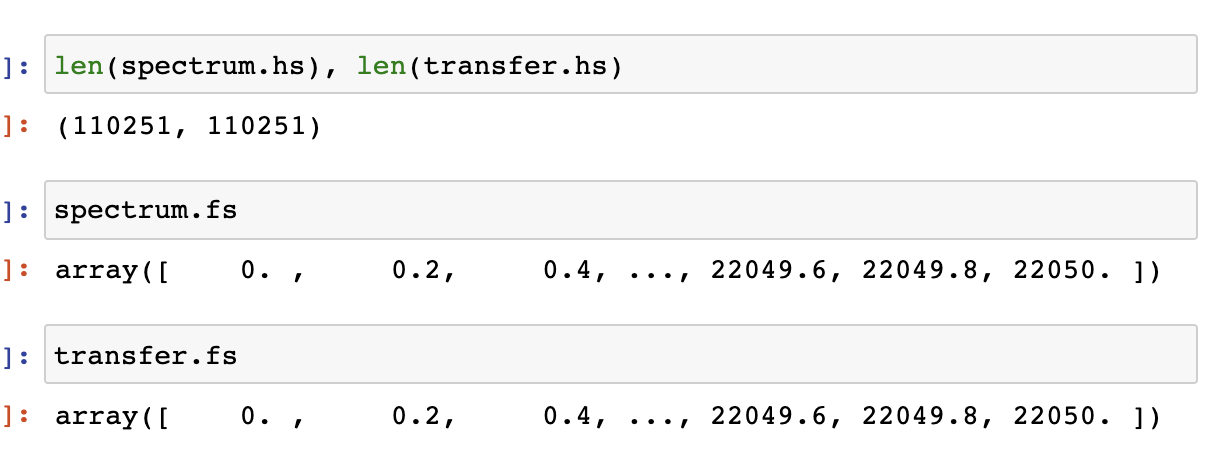
\includegraphics[width=0.75\textwidth]{13.png}
        \caption{2}
        \label{fig:first}
\end{figure}

Рисунок ниже дает нам представление о том, с чем мы имеем дело, хотя и немного неточно.

\begin{figure}[H]
        \centering
        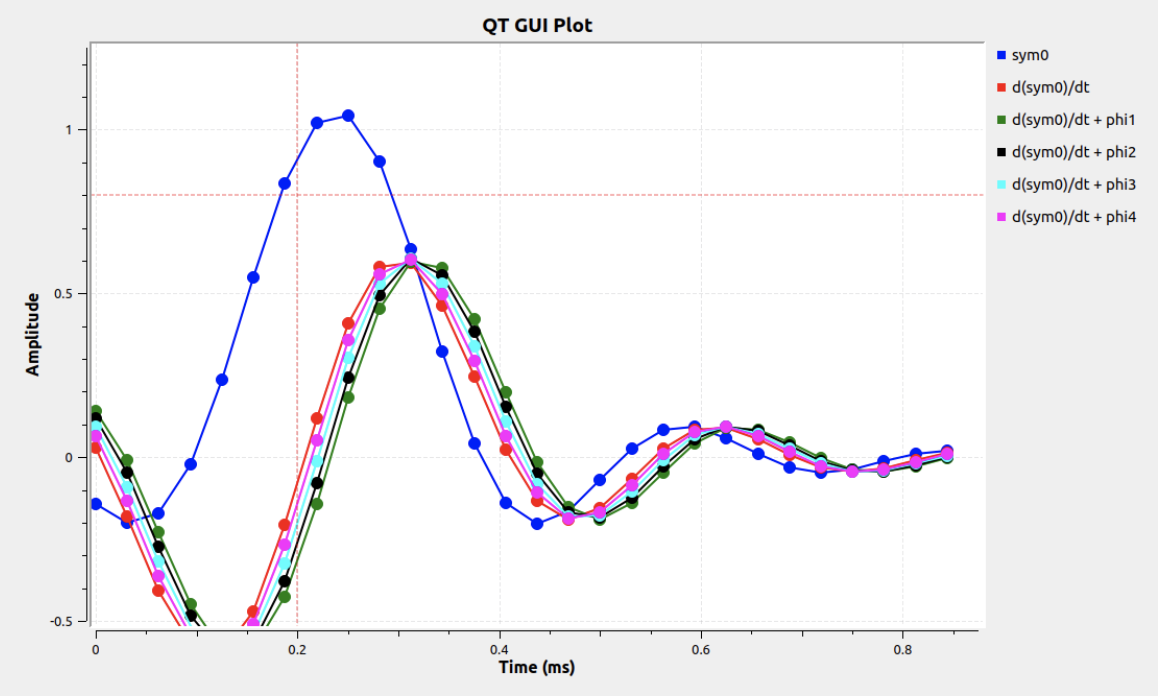
\includegraphics[width=0.75\textwidth]{14.png}
        \caption{2}
        \label{fig:first}
\end{figure}

Но, как мы уже обсуждали, это только смоделированное приближение; в действительности выборки каждого фильтра не будут происходить в один и тот же момент времени. Мы должны увеличить выборку по количеству фильтров (например, 5), чтобы действительно увидеть это поведение. Однако это может подсказать нам, что происходит дальше. Мы можем рассматривать эти разные фильтры как части одного большого фильтра с избыточной дискретизацией M, где M = 5 в нашем простом примере. Мы могли бы повысить дискретизацию нашего входящего сигнала на эту величину и выбрать момент времени, когда мы получим выходной сигнал 0 разностного фильтра. Проблема в том, что мы говорим о большом количестве дополнительной вычислительной сложности, поскольку она пропорциональна нашей частоте дискретизации. Вместо этого мы работаем над фильтрами разных фаз на входящей частоте дискретизации, но с их банком на этих разных фазах,

\section{Использование блока многофазной синхронизации:}

Теперь давайте используем этот блок в нашей симуляции. Пример потокового графа mpsk_stage3.grc принимает выходные данные модели канала и передает их через наш блок Polyphase Clock Sync. Этот блок настроен с 32 фильтрами по причинам, которые мы обсуждали выше, и полосой пропускания петли 2pi / 100. Блок также принимает значение для ожидаемых выборок на символ, но это всего лишь наше предположение о том, каким, по нашему мнению, должно быть это значение. Внутри блок адаптируется к этому значению в зависимости от скорости входящего сигнала. Обратите внимание, однако, что я установил эту симуляцию там, где оценка немного отличается от 4 sps, с которыми мы передаем. Это сделано для имитации начального временного сдвига между передатчиком и приемником, поскольку мы инициализируем наш элемент управления Timing Offset равным 1.0.

\begin{figure}[H]
        \centering
        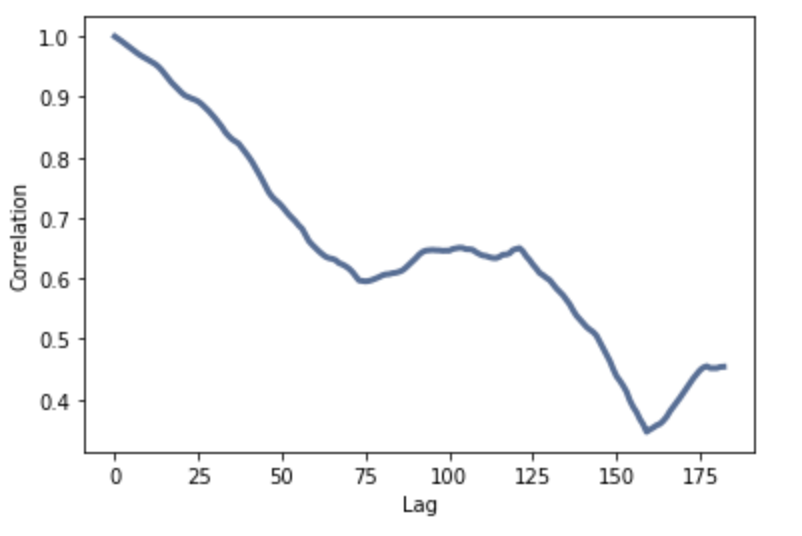
\includegraphics[width=0.75\textwidth]{15.png}
        \caption{2}
        \label{fig:first}
\end{figure}

\begin{figure}[H]
        \centering
        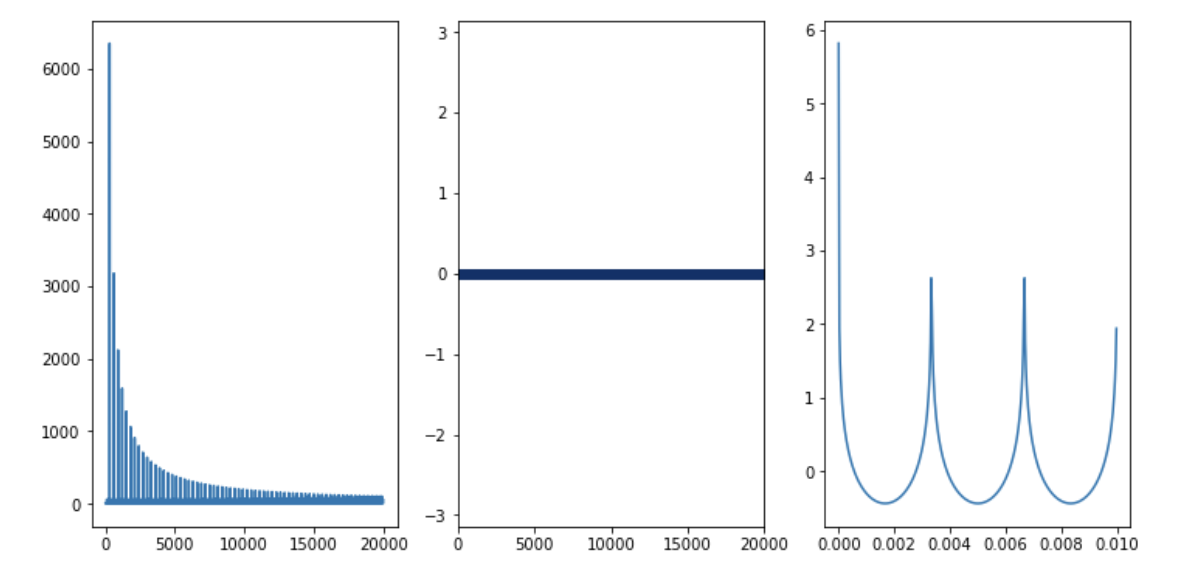
\includegraphics[width=0.75\textwidth]{16.png}
        \caption{2}
        \label{fig:first}
\end{figure}

При запуске этого скрипта мы видим созвездие слева как полученный сигнал до восстановления синхронизации и справа после восстановления синхронизации. Это все еще немного шумно из-за ISI после 32 фильтров, который быстро поглощается шумом, когда мы устанавливаем значение параметра Noise Voltage больше 0.

Затем мы можем поиграть с изменением временного и частотного смещения. Перемещение шкалы времени показывает нам, как блок синхронизации часов удерживает сигнал синхронизированным по времени и выводит отсчеты в идеальных точках созвездия (или очень близко к ним). Когда мы добавляем частотный сдвиг, мы видим, что созвездие становится кругом. Созвездие все еще находится на единичном круге, поэтому мы знаем, что оно все еще сохраняет правильную синхронизацию, но блок не позволяет нам корректировать смещение частоты.

\section{Многолучевость:}

Воздействие комбинации этих сигналов на приемник - искажение сигнала. Если разница во времени между отражениями достаточно мала по сравнению с шириной символа, искажение может быть внутри символа - внутрисимвольная интерференция. Когда отражения длиннее времени символа, отражение от одного символа будет влиять на следующие сигналы - еще одна причина межсимвольной интерференции.

Нам нужно исправить это поведение, и мы можем сделать это, используя механизм, очень похожий на стереоэквалайзер. Фактически мы называем их эквалайзерами. С помощью стереофонического эквалайзера мы можем изменить усиление определенных частот, чтобы либо подавить, либо усилить эти сигналы, наиболее распространенными из которых являются низкие и высокие частоты. Я создал очень простой пример под названием multipath_sim.grc, чтобы помочь нам изучить, как это выглядит в частотной области.

\begin{figure}[H]
        \centering
        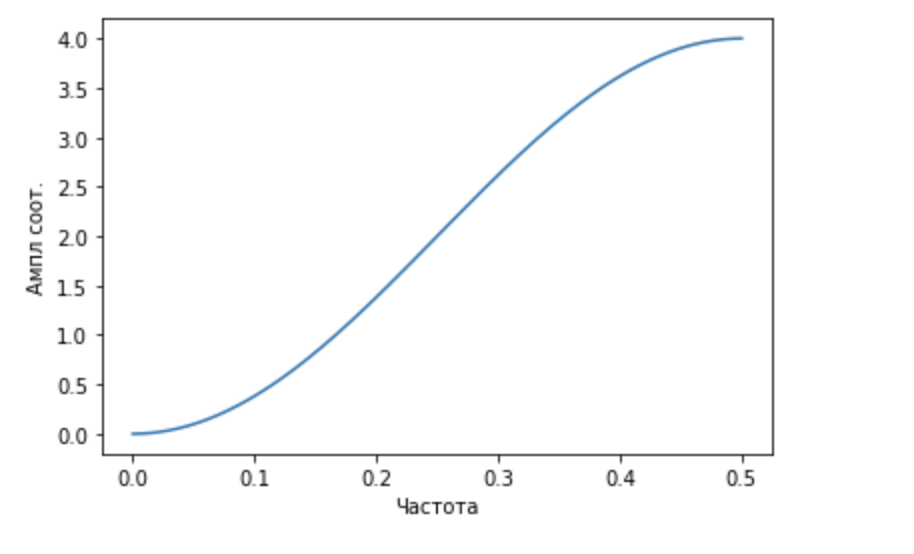
\includegraphics[width=0.75\textwidth]{17.png}
        \caption{2}
        \label{fig:first}
\end{figure}

Это моделирование настраивает модель канала, чтобы предоставить каналу пять элементов управления эквалайзером, четыре из которых мы можем изменить. Эти элементы управления настроены одинаково по частоте, и мы можем настроить их от 0 до 1. При значении 1 элемент управления позволит этим частотам проходить без помех. При значении 0 они будут производить глубокий нуль в спектре, который повлияет на все частоты вокруг него. График частоты установлен на среднее значение.

\begin{figure}[H]
        \centering
        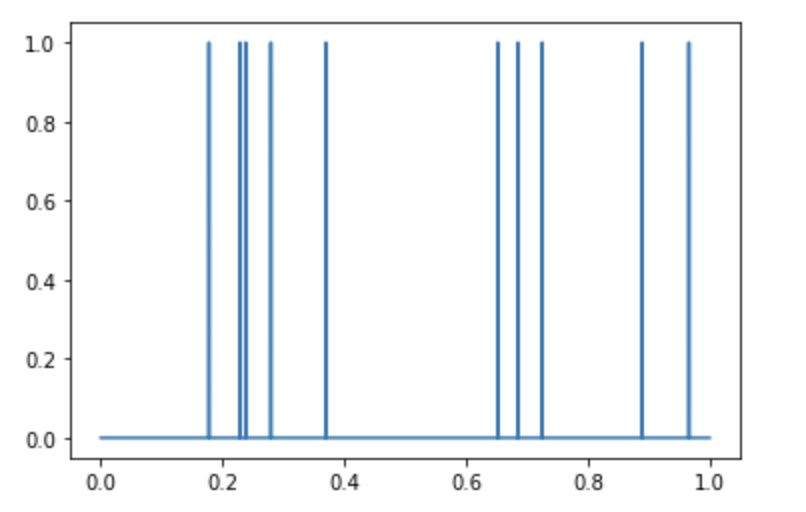
\includegraphics[width=0.75\textwidth]{18.png}
        \caption{2}
        \label{fig:first}
\end{figure}

\section{Эквалайзеры:}

Алгоритм CMA принимает количество касаний для использования в эквалайзере, которое будет основано на некоторой комбинации обоснованного предположения, известных передовых практик и, возможно, некоторых фактических знаний о самом канале. Мы хотим, чтобы это число оставалось небольшим, чтобы уменьшить накладные расходы на алгоритм, обеспечивая при этом достаточное количество степеней свободы для корректировки нашего канала.

В примере mpsk_stage4.grc мы используем алгоритм CMA с 11 нажатиями.

\begin{figure}[H]
        \centering
        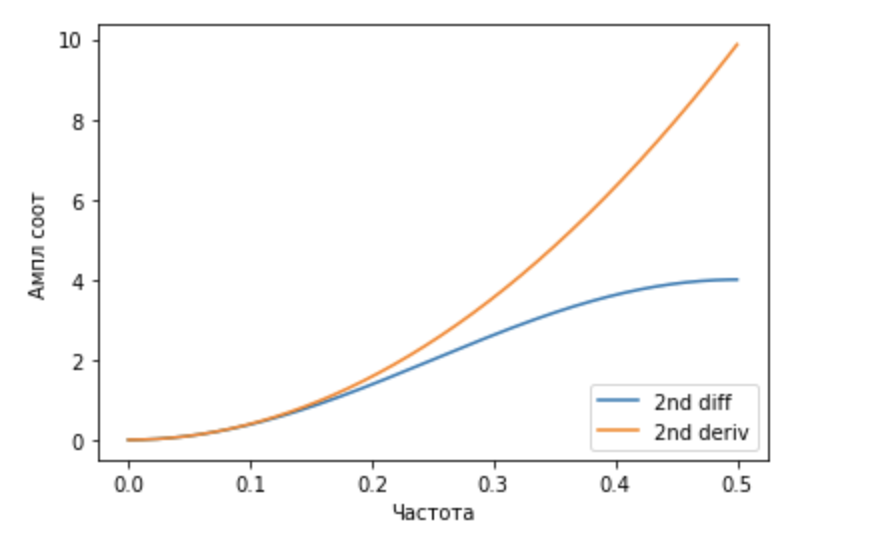
\includegraphics[width=0.75\textwidth]{19.png}
        \caption{2}
        \label{fig:first}
\end{figure}

Мы можем наблюдать сходимость алгоритма CMA. Также обратите внимание, что, поскольку у нас есть и тактовая синхронизация, и блок эквалайзера, они сходятся независимо, но один этап будет влиять на следующий этап.

\begin{figure}[H]
        \centering
        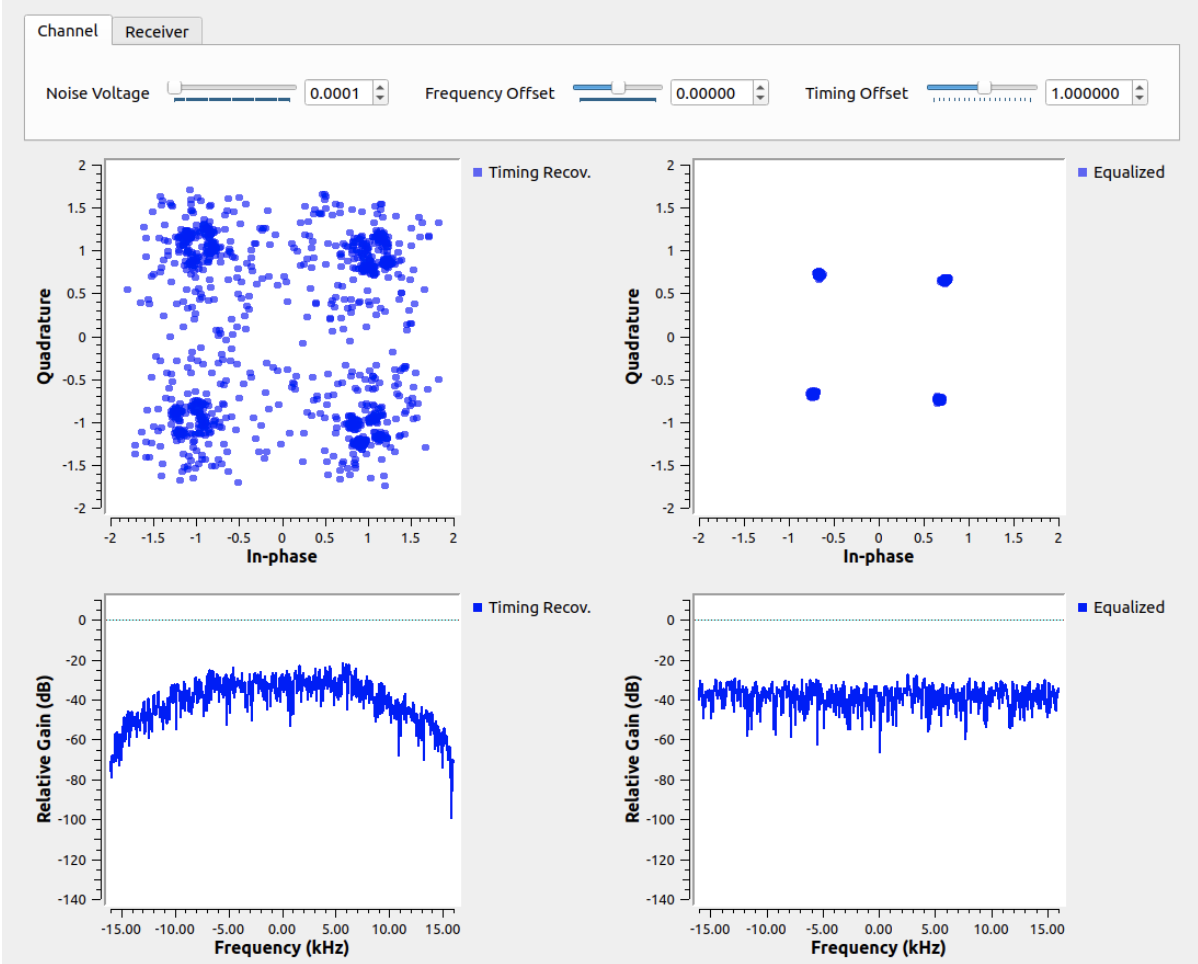
\includegraphics[width=0.75\textwidth]{20.png}
        \caption{2}
        \label{fig:first}
\end{figure}

\section{Фазовая и точная частотная коррекция:}

Учитывая, что мы выровняли канал, у нас все еще есть проблема смещения фазы и частоты. Эквалайзеры, как правило, не адаптируются быстро, поэтому смещение частоты может быть легко за пределами возможностей эквалайзера. Кроме того, если мы просто запускаем эквалайзер CMA, все, о чем он заботится, - это схождение к единичной окружности. Он ничего не знает о созвездии, поэтому, когда он блокируется, он блокируется на любой заданной фазе. Теперь нам нужно исправить любой сдвиг фазы, а также любой сдвиг частоты.

Две вещи об этом этапе. Во-первых, мы будем использовать цикл второго порядка, чтобы мы могли отслеживать как фазу, так и частоту (которая является производной от фазы) во времени. Во-вторых, тип восстановления, с которым мы будем иметь дело, предполагает, что мы выполняем точную коррекцию частоты. Поэтому мы должны быть уверены, что мы уже находимся в приличном диапазоне идеальной частоты. Если мы будем слишком далеко, наш цикл здесь не сойдется, и мы продолжим вращаться. Есть способы сделать грубую коррекцию частоты, но мы не будем вдаваться в подробности.

Для этой задачи мы собираемся использовать цикл Костаса в примере mpsk_stage5.grc (здесь также можно использовать Constellation Receiver ). Блок Costas Loop может синхронизировать BPSK, QPSK и 8PSK. Приемник созвездия будет привязан к любому заданному объекту созвездия, хотя в зависимости от созвездия функция принятия решения может быть более или менее сложной.

\begin{figure}[H]
        \centering
        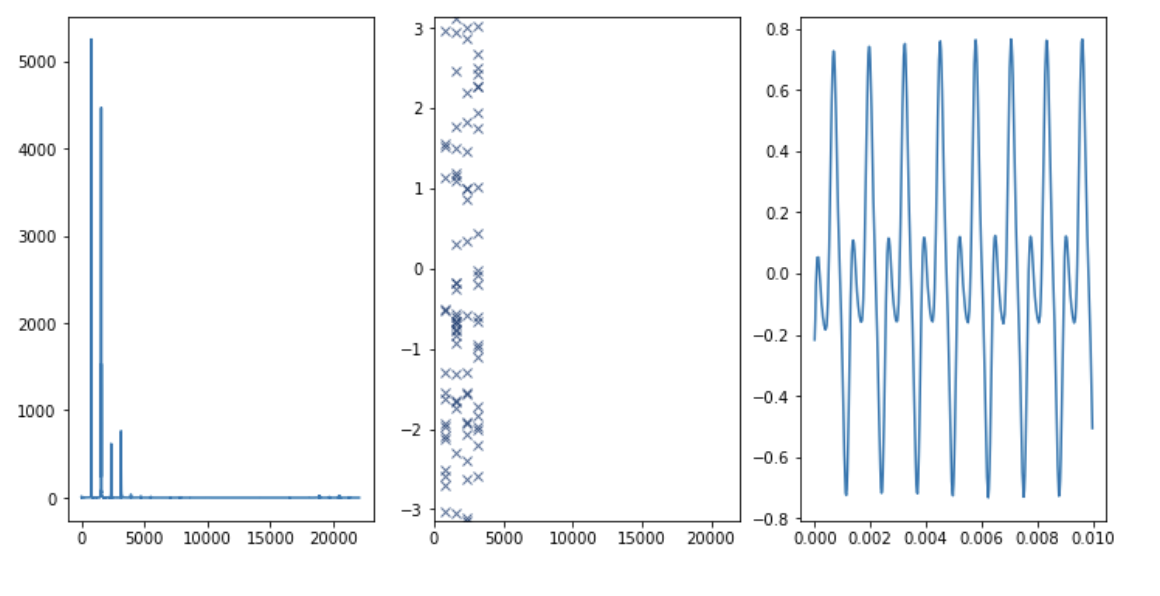
\includegraphics[width=0.75\textwidth]{21.png}
        \caption{2}
        \label{fig:first}
\end{figure}

Этот блок, как и все наши другие, использует цикл второго порядка и поэтому определяется параметром полосы пропускания цикла. Еще ему необходимо знать порядок модуляции PSK: 2 для BPSK, 4 для QPSK и 8 для 8PSK. На следующем изображении мы установили шум, временной сдвиг, простой многолучевой канал и частотный сдвиг. После эквалайзера мы видим, что все символы находятся на единичном круге, но вращаются из-за сдвига частоты, который еще не исправляется. На выходе блока цикла Костаса мы можем видеть заблокированное созвездие, как мы начали, плюс дополнительный шум, с которым мы ничего не можем поделать.

\begin{figure}[H]
        \centering
        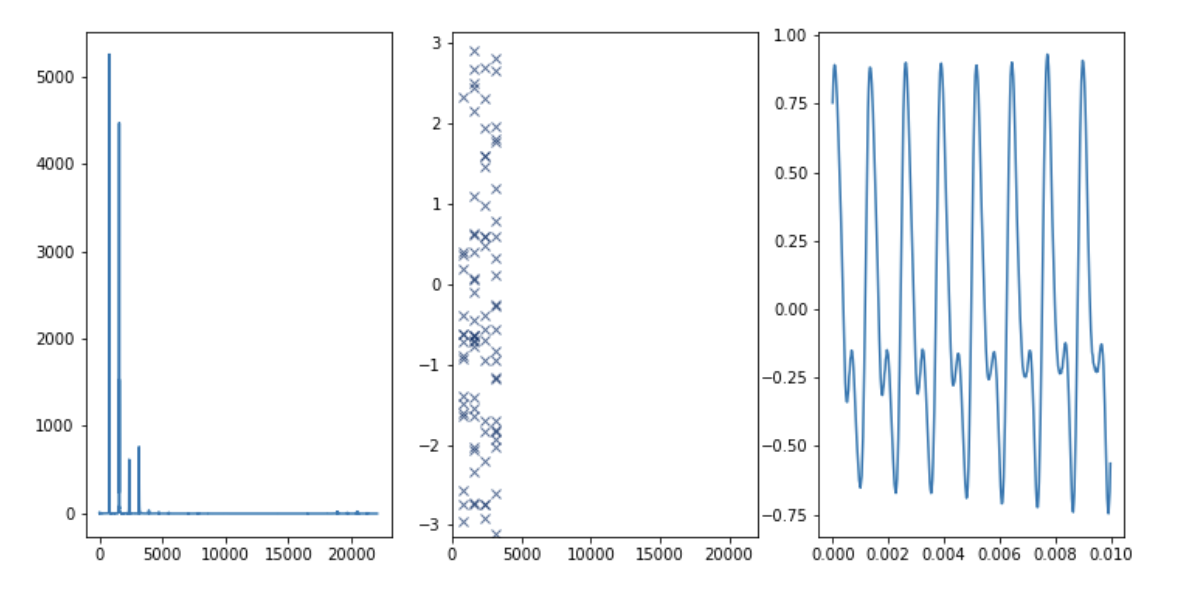
\includegraphics[width=0.75\textwidth]{22.png}
        \caption{2}
        \label{fig:first}
\end{figure}

\section{Расшифровка:}

Теперь, когда самая сложная часть сделана, мы можем декодировать сигнал. Используя пример потокового графа mpsk_stage6.grc, мы вставляем Constellation Decoder после цикла Костаса, но наша работа еще не завершена. На этом этапе мы получаем наши символы от 0 до 3, потому что это размер нашего алфавита в схеме QPSK. Но из этих символов 0–3, как мы можем точно знать, что у нас есть такое же отображение символов на точки созвездия, которое мы делали при передаче? Обратите внимание в нашем обсуждении выше, что мы ничего не делали, не имея никаких сведений о переданном преобразовании символа в созвездие, что означает, что у нас может быть неоднозначность в 90 градусов в созвездии. К счастью, мы избежали этой проблемы, передав дифференциальные символы. На самом деле мы не передавали само созвездие, мы передавали разницу между символами созвездия, установив для параметра Differential в блоке Constellation Modulator значение True. 

\begin{figure}[H]
        \centering
        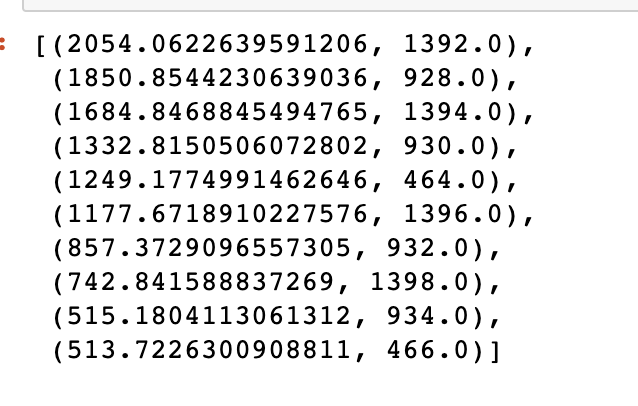
\includegraphics[width=0.75\textwidth]{23.png}
        \caption{2}
        \label{fig:first}
\end{figure}

Блок-граф использует блок дифференциального декодера для преобразования кодированных дифференциальным кодом символов обратно в их исходные символы из-за фазовых переходов, а не самой абсолютной фазы. Но даже отсюда наши символы не совсем правильные. На самом деле, это самая сложная часть демодуляции. На этапах синхронизации на нашей стороне были основы физики и математика. Однако теперь мы должны интерпретировать какой-то символ, основываясь на том, что кто-то сказал о нем. Нам, по сути, просто нужно знать это отображение. К счастью, мы это делаем, поэтому мы используем блок Map для преобразования символов из дифференциального декодера в исходные символы, которые мы передали. На данный момент у нас теперь есть исходные символы от 0 до 3, поэтому давайте распакуем эти 2 бита на символ в биты, используя биты распаковки.блокировать. Теперь у нас есть исходный битовый поток данных!

Но как мы узнаем, что это исходный битовый поток? Для этого мы сравним с входным битовым потоком, что мы можем сделать, потому что это моделирование и у нас есть доступ к переданным данным. Но, конечно, передатчик произвел упакованные биты , поэтому мы снова используем битовый блок распаковки для распаковки с 8 бит на байт до 1 бита на байт. Затем мы конвертируем эти потоки в значения 0,0 и 1,0 с плавающей запятой просто потому, что наши приемники времени принимают только значения с плавающей запятой и комплексные значения. Сравнение этих двух напрямую не покажет нам ... ничего. Почему? Поскольку в цепочке приемника много блоков и фильтров, которые задерживают сигнал, принятый сигнал отстает на некоторое количество бит. Чтобы компенсировать это, мы должны задерживать переданные биты на ту же величину, используя Delayблокировать. Затем вы можете настроить задержку, чтобы найти правильное значение и посмотреть, как синхронизируются биты. Вы также можете вычесть один сигнал из другого, чтобы увидеть, когда они синхронизированы, поскольку на выходе будет 0. Добавление шума и других влияний на канал можно легко увидеть как битовые ошибки, если этот сигнал не равен 0. Примечание: подождите несколько секунд после каждое изменение значения задержки.

\begin{figure}[H]
        \centering
        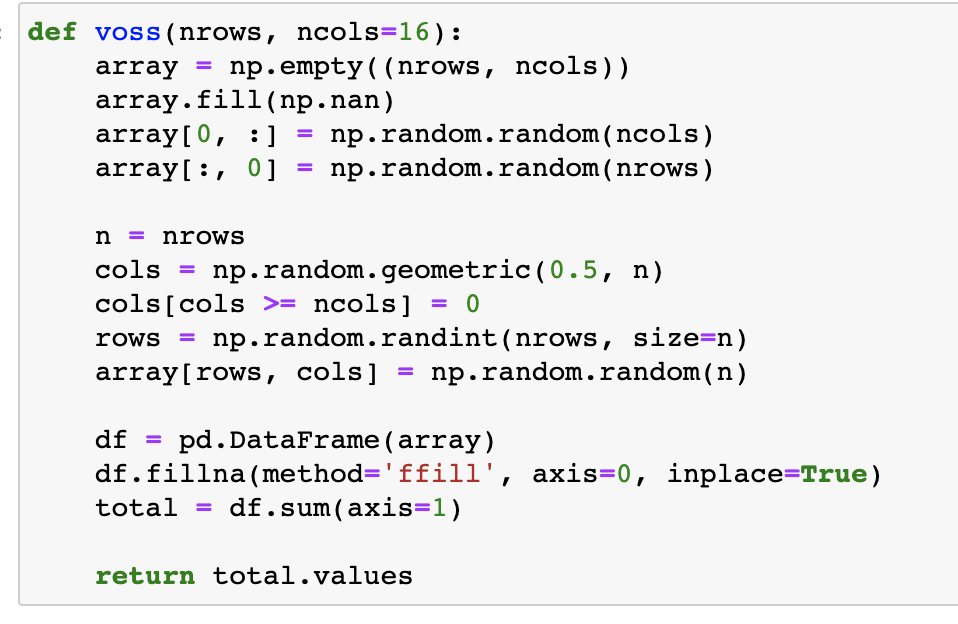
\includegraphics[width=0.75\textwidth]{24.png}
        \caption{2}
        \label{fig:first}
\end{figure}

\end{document}
